\chapter{RESULTADOS DE SIMULAÇÕES}
\label{resultados}
\section{\textbf{Introdução}}
Neste capítulo serão apresentadas as simulações realizadas para analisar o comportamento de partículas presentes em turbomáquinas em ação.
Foram escolhidos cinco tipos de geometria para serem simulados:
\begin{itemize}
    \item \textbf{Canal reto}.

        Uma geometria simples, que busca simular o comportamento básico das partículas sobre efeito de um escoamento. 
        A malha utilizada tem $1072$ elementos definidos sobre $593$ nós, exposta na \ref{channel_mesh}.
        \begin{figure}[H]
            \centering
            \stackunder{
                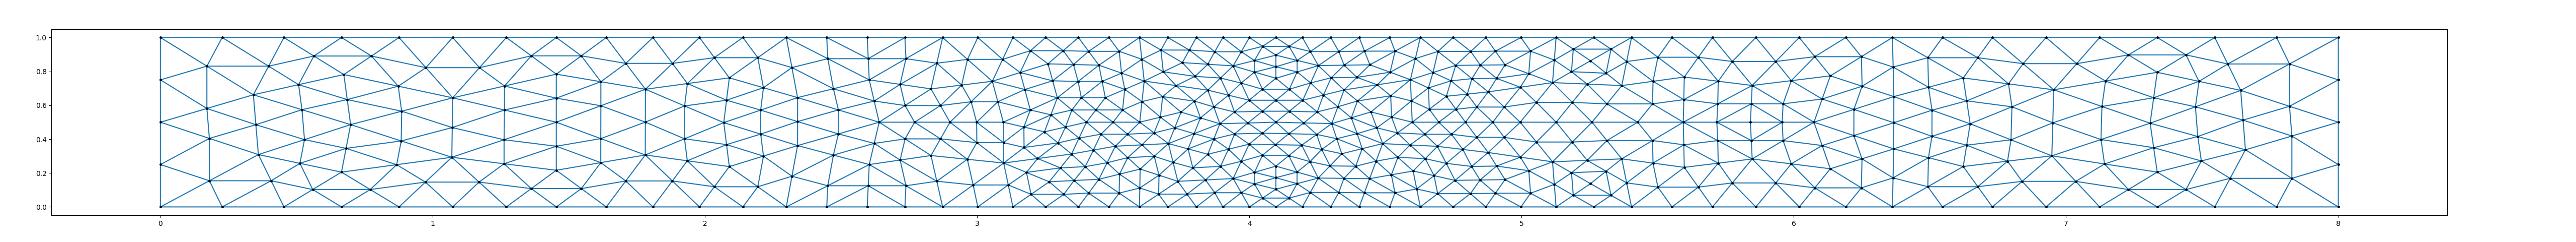
\includegraphics[width=\linewidth]{figures/Channel_mesh.png}
            } {\raggedleft \scriptsize Fonte: Autor.}
            \caption{Malha da simulação em um canal reto.}
            \label{channel_mesh}
        \end{figure}

    \item \textbf{Canal com um obstáculo circular no centro}.

        Esta geometria visa simular o efeito de obstáculos, ou até mesmo as próprias partículas no escoamento.
        Porém, não é utilizada neste trabalho a implementação \textit{two-way}, que levaria em conta os efeitos das partículas no escoamento.
        Neste caso a simulação foi aplicada a uma malha de $868$ elementos e $494$ nós.
        \begin{figure}[H]
            \centering
            \stackunder{
                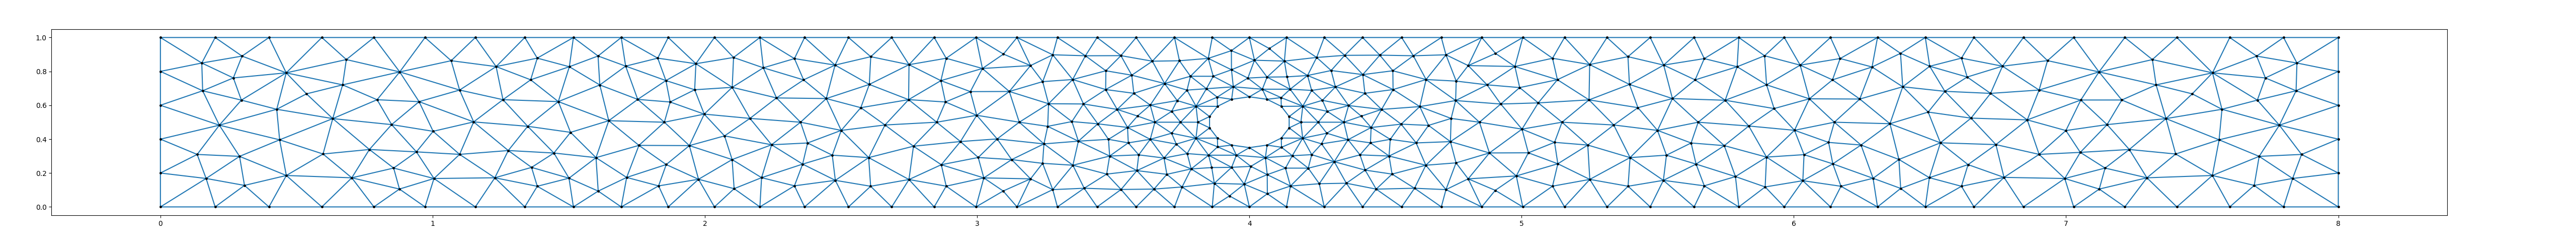
\includegraphics[width=\linewidth]{figures/Obstacle_mesh.png}
            } {\raggedleft \scriptsize Fonte: Autor.}
            \caption{Malha da simulação em um canal com um obstáculo.}
            \label{obstacle_mesh}
        \end{figure}

    \item \textbf{Canal com degrau}.

        O escoamento em um canal com um degrau, ou uma diferença brusca de percurso, possui diversos efeitos interessantes para serem observados.
        Como por exemplo nas regiões de curva, pode fazer-se observações sobre o comportamento em conexões de tubulações reais.
        Com uma malha de $676$ elementos definidos sobre $380$ nós.
        \begin{figure}[H]
            \centering
            \stackunder{
                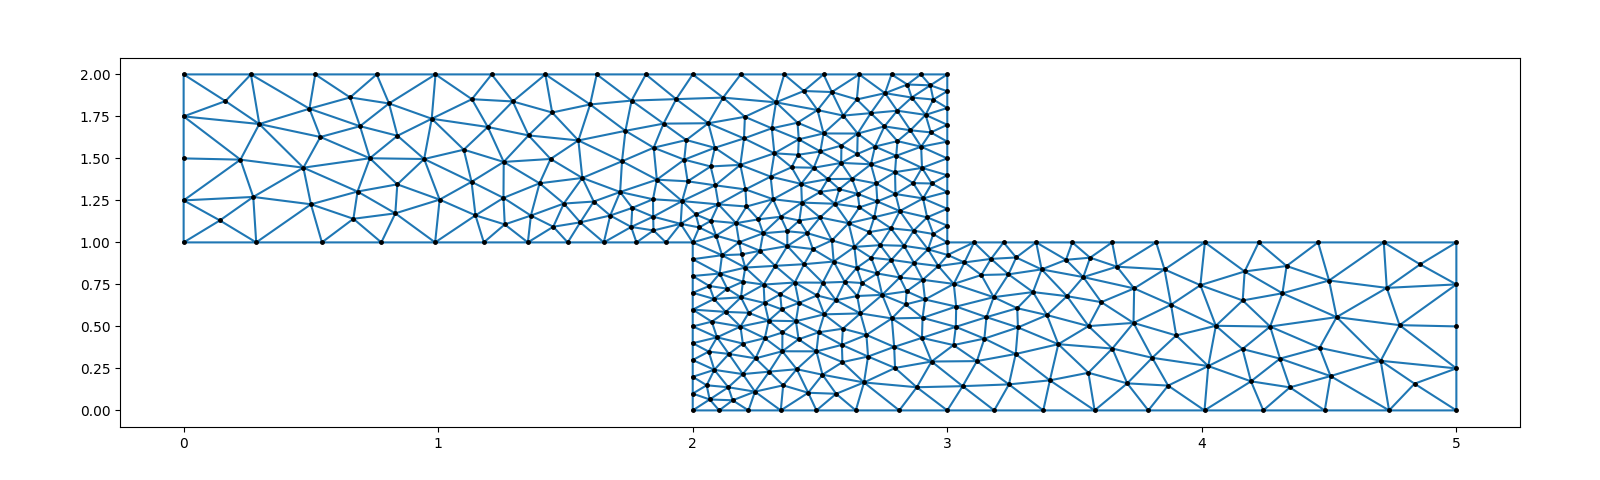
\includegraphics[width=\linewidth]{figures/Step_mesh.png}
            } {\raggedleft \scriptsize Fonte: Autor.}
            \caption{Malha da simulação em um canal com degrau.}
            \label{step_mesh}
        \end{figure}

    \item \textbf{Canal com restrição}.

        O escoamento em um canal com restrição demonstra os efeitos da redução de seção transversal.
        Um exemplo deste tipo de escoamento seria em medidores de vazão, como o Tubo de Venturi. 
        Sua malha foi criada com $1047$ elementos definido distribuidos sobre $600$ nós:
        \begin{figure}[H]
            \centering
            \stackunder{
                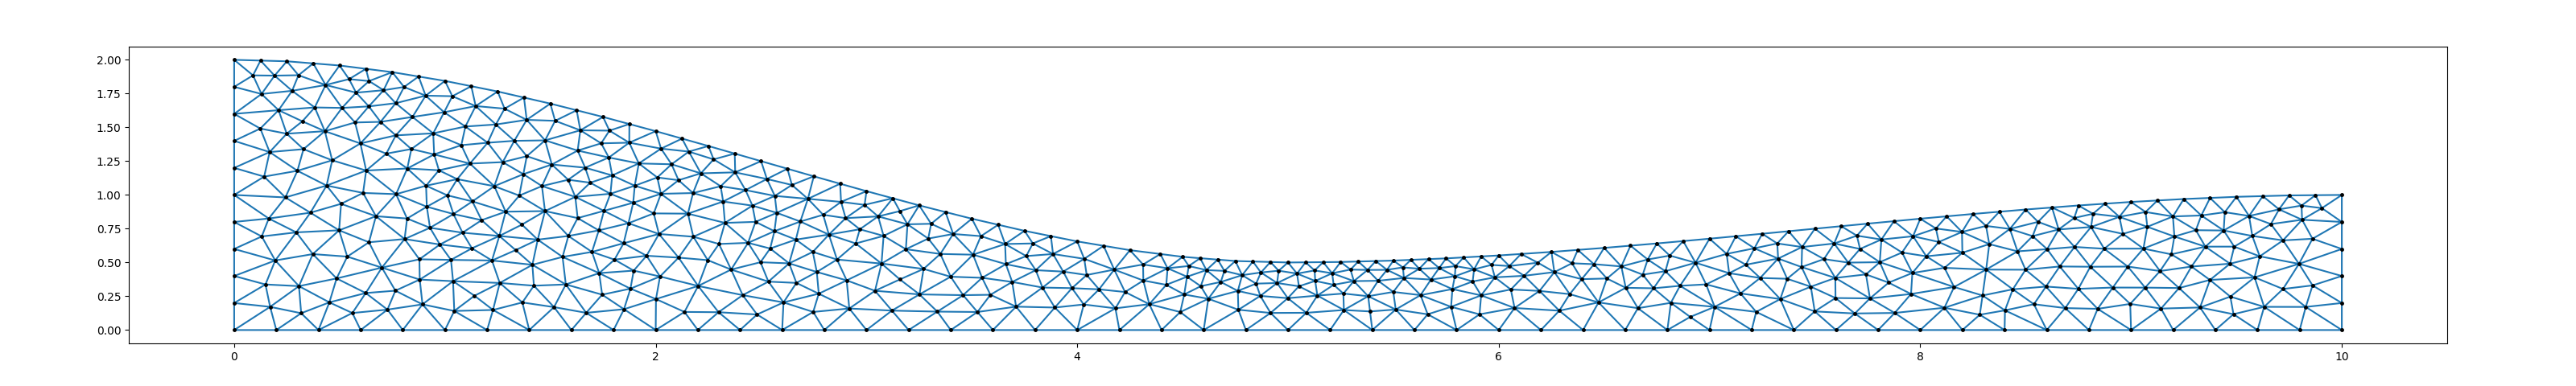
\includegraphics[width=\linewidth]{figures/Nozzle_mesh.png}
            } {\raggedleft \scriptsize Fonte: Autor.}
            \caption{Malha da simulação em um canal com restrição.}
            \label{nozzle_mesh}
        \end{figure}

    \item \textbf{Pá de um rotor}.

        Finalmente, será analizado o comportamento de partículas em um escoamento presente em uma seção de um rotor de uma turbomáquina.
        Neste trabalho, foi tomado um referencial estacionário na pá, sem efeito da rotação do rotor no escoamento.
        Foi utilizada uma malha de $1058$ elementos definidos sobre $531$ nós.
        \begin{figure}[H]
            \centering
            \stackunder{
                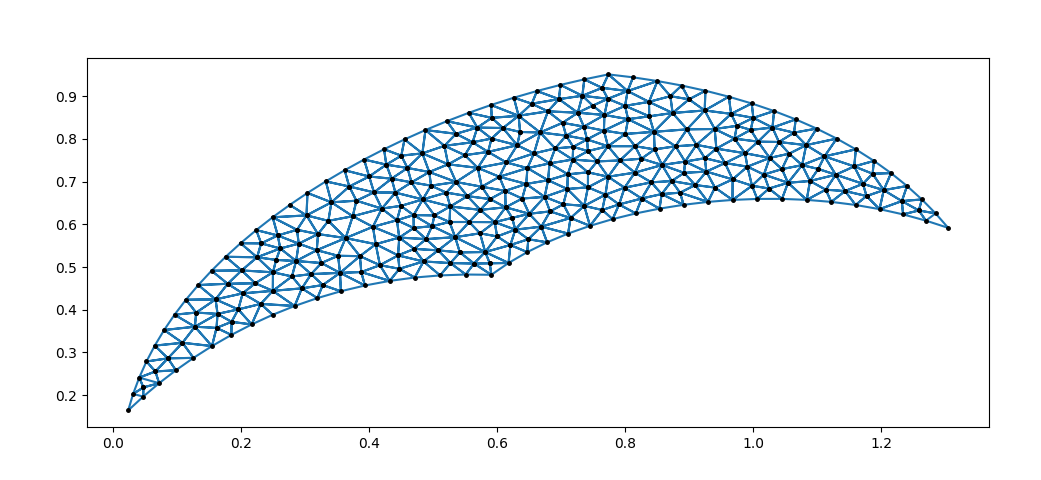
\includegraphics[width=\linewidth]{figures/Rotor_mesh.png}
            } {\raggedleft \scriptsize Fonte: Autor.}
            \caption{Malha da simulação em uma pá de um rotor.}
            \label{rotor_mesh}
        \end{figure}
\end{itemize}

Foi utilizado o software ParaView para exibição dos gráficos de resultados.
A escala das figuras mostra o valor da magnitude da velocidade em cada nó.

Em cada simulação, com exceção das simulações na palheta de um rotor, são inseridas cinco partículas de ouro perfeitamente rígidas, igualmente espalhadas, com $d_p=1mm=1.10^{-3}m$ de diâmetro e densidade de $\rho_p=20000kg/m^3$.
Estas partículas estão submersas em um fluido ideal com características: $\mu_f=50kg/m.s$ de viscosidade dinâmica e densidade de $\rho_f=50kg/m^3$, para que trabalhe em uma situação com número de Reynolds reduzido, e menor que a restrição da equação BBO\ref{sec_eq_part}.

As partículas são iniciadas com velocidade nula e em posições próximas à entrada do escoamento, porém fora de sua região de transição.
As simulações foram executadas para um tempo total de $5s$ com um tempo entre cálculos de $dt=3.33e^{-5}s$.
O trajeto de cada partícula é exibido com uma cor diferente para auxiliar a interpretação. 

%------------------- Canal Reto-------------------------------
\section{\textbf{Simulação Em Um Canal Reto}}
\label{sec_channel}
O escoamento em um canal reto permite vizualizar o movimento livre das partículas sob efeito do fluido.
A sua configuração é similar ao exemplo de Poiseuille \ref{sec_poiseuille}.
As condições do escoamento são de um comprimento $L=8m$ com altura constante de $D=1m$, o fluido entra com velocidade constante pela região da esquerda com velocidade $\vec{v}_{ent}=(1, 0)m/s$.
Nas paredes há a condição de não escorregamento, portanto a velocidade nas paredes inferior e superior são nulas, $\vec{v}_{sup}=\vec{v}_{inf}=0$.
A corrente possui uma condição de contorno variando de $0$ a $1$ nas bordas de acordo com sua posição, equivalente a $\psi_{cc}=y$.

Seu campo de velocidades é apresentado na \ref{channel_result}:
\begin{figure}[H]
    \centering
    \stackunder{
        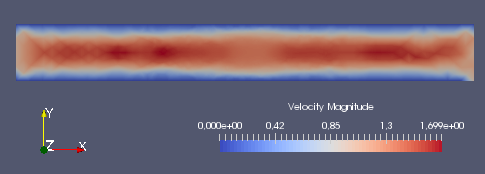
\includegraphics[width=\linewidth]{figures/Channel_result.png}
    } {\raggedleft \scriptsize Fonte: Autor.}
    \caption{Campo de velocidades de um escoamento em um canal reto.}
    \label{channel_result}
\end{figure}

A trajetória das partículas pode ser analizada na \ref{channel_trajectory}:
\begin{figure}[H]
    \centering
    \stackunder{
        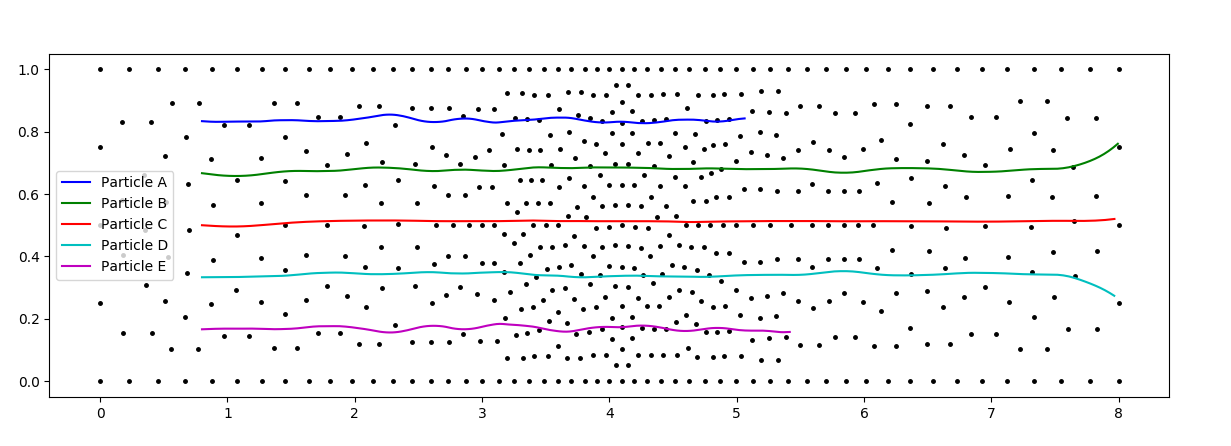
\includegraphics[width=\linewidth]{figures/Channel_particle_trajectory.png}
    } {\raggedleft \scriptsize Fonte: Autor.}
    \caption{Trajeto de partículas inseridas em um escoamento em um canal reto.}
    \label{channel_trajectory}
\end{figure}

Pode-se observar que as partículas seguem o escoamento como esperado, com uma diferença de distância no percurso causado pelo perfil de velocidades.
Na região de saída, as partículas tendem a se espalhar devido às condições de contorno na região.

%------------------- Obstaculo -------------------------------
\section{\textbf{Simulação Em Um Canal Com Obtáculo}}
\label{sec_obstacle}
Em um escoamento com obtáculo, pode-se observar o efeito do obstáculo no campo de velocidades do escoamento, assim como o comportamento das partículas ao interagir com este obstáculo.

Novamente, as condições do escoamento são iguais a simulação anterior \ref{sec_channel}, porém com as condições de contorno aplicadas também a região do obstáculo.
Onde $\vec{v}_{obstaculo}=0$ e $\psi_{obstaculo}=y$.

Para auxiliar na visualização do resultado, é exibido em conjunto da velocidade as linhas de corrente do campo, desenhadas com o auxílio de uma ferramenta de desenho das curvas de nível.
Observa-se a distorção no campo de velocidades causada pelo obstáculo na \ref{obstacle_result}:
\begin{figure}[H]
    \centering
    \stackunder{
        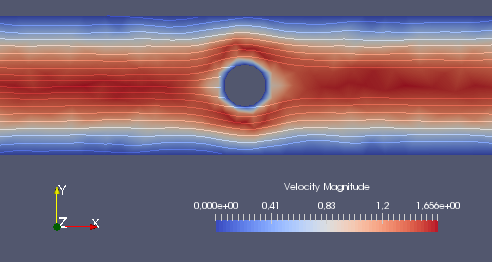
\includegraphics[width=\linewidth]{figures/Obstacle_result.png}
    } {\raggedleft \scriptsize Fonte: Autor.}
    \caption{Campo de velocidades de um escoamento com obstáculo.}
    \label{obstacle_result}
\end{figure}

E as partículas realizam percursos apresentados na \ref{obstacle_trajectory}:
\begin{figure}[H]
    \centering
    \stackunder{
        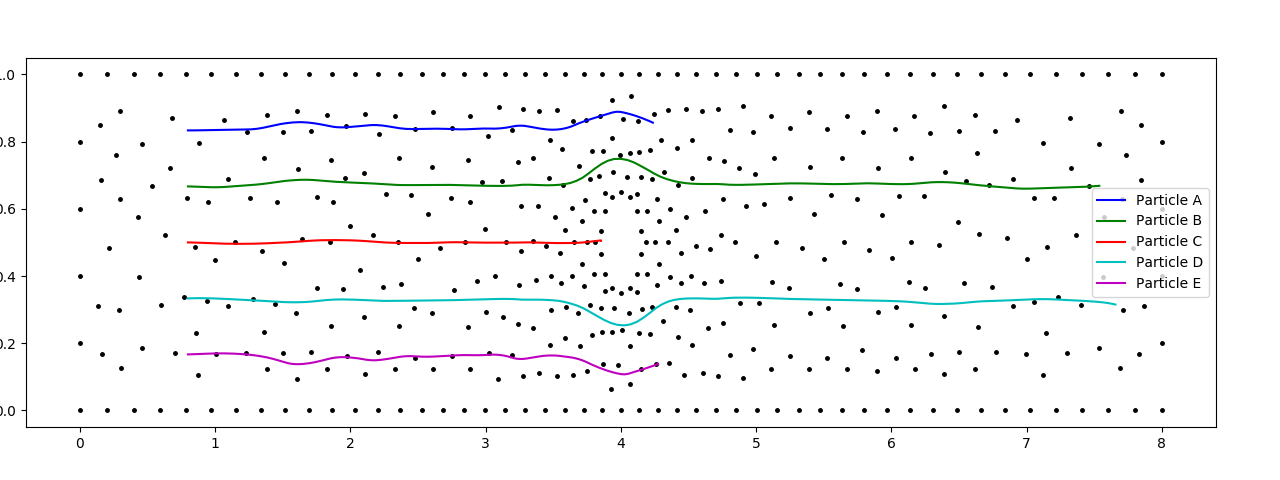
\includegraphics[width=\linewidth]{figures/Obstacle_particle_trajectory.png}
    } {\raggedleft \scriptsize Fonte: Autor.}
    \caption{Trajeto de partículas inseridas em um escoamento com obstáculo.}
    \label{obstacle_trajectory}
\end{figure}

Nesta simulação pode-se observar o efeito do obstáculo que desvia o trajeto das partículas e a colisão de uma delas, que fica retida devido as correntes de velocidade nulas na condição de contorno das paredes.

%------------------- Step ------------------------------------
\section{\textbf{Simulação Em Um Canal Com Degrau}}
\label{sec_step}
No escoamento com degrau há um desvio no trajeto que tende a causar colisões das partículas devio a inércia de seu movimento.
Dependendo de suas características, as partículas estão mais propensas a colidirem com a parede direita superior ou serão mais influenciadas pelo fluido e terão sua trajetória alterada.

Para este escoamento são adaptadas as condições anteriores para a geometria de um comprimento $L=5m$ com altura de entrada e saída de $D=1m$, o fluido entra com velocidade constante pela região da esquerda com velocidade $\vec{v}_{ent}=(1, 0)m/s$.
Nas paredes há a condição de não escorregamento, portanto a velocidade nas paredes são nulas, $\vec{v}_{parede}=0$.
A corrente possui uma condição de contorno variando de $0$ a $1$ onde ela é $0$ para as paredes inferiores e $1$ para as superiores.
E na região vertical esquerda de entrada toma-se a corrente como $\psi_{cc}=y-1$, e $\psi_{cc}=y$ na região vertical direita de saída.

Novamente, são incluidas as curvas de nível da velocidade na exibição do campo de velocidades na \ref{step_result}:
\begin{figure}[H]
    \centering
    \stackunder{
        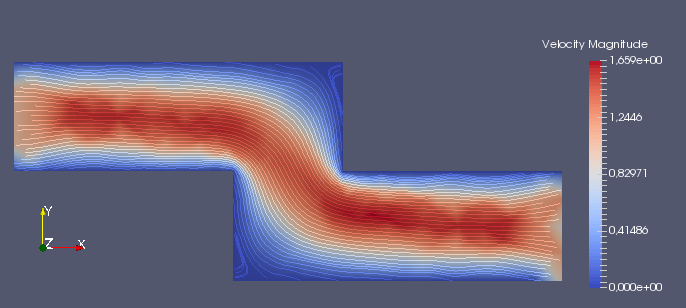
\includegraphics[width=\linewidth]{figures/Step_result.png}
    } {\raggedleft \scriptsize Fonte: Autor.}
    \caption{Campo de velocidades de um escoamento com degrau.}
    \label{step_result}
\end{figure}

Como outra forma de visualizar o campo de velocidades, são exibidas as velocidades nos nós como vetores em um diagrama de flechas ou \textit{quiver plot}:
\begin{figure}[H]
    \centering
    \stackunder{
        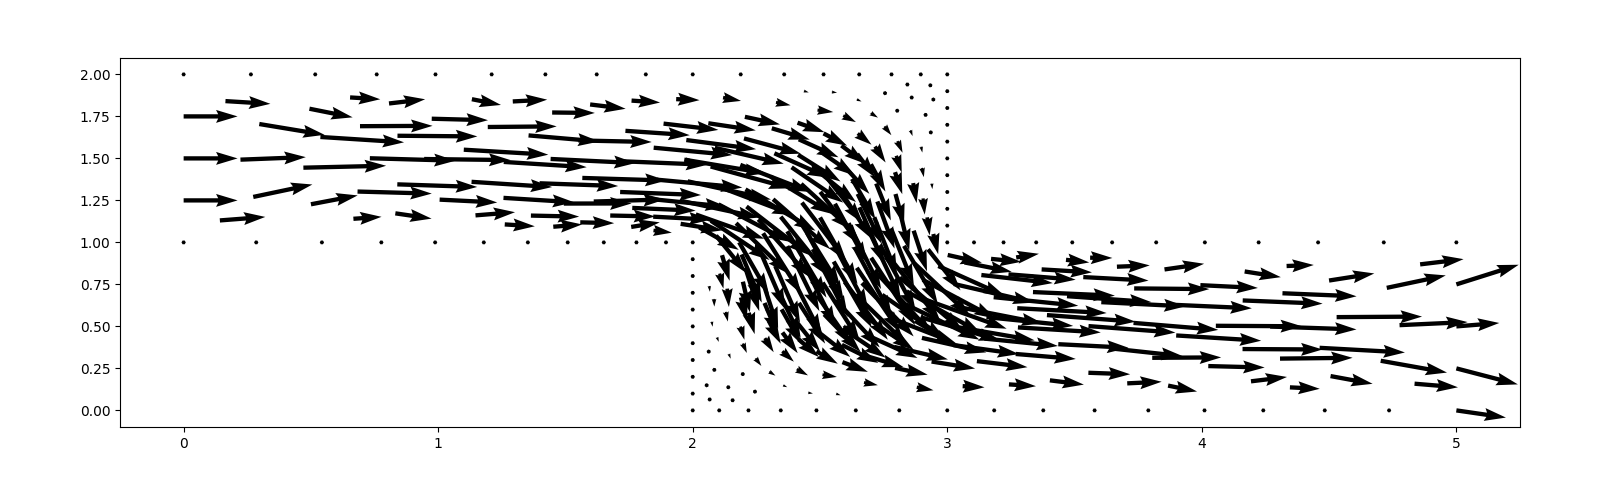
\includegraphics[width=\linewidth]{figures/Step_velocity_field.png}
    } {\raggedleft \scriptsize Fonte: Autor.}
    \caption{Vetores de velocidades de um escoamento com degrau.}
    \label{step_velocity}
\end{figure}

As curvas dos trajetos percorridos pelas partículas nesta simulação são apresentados na \ref{step_trajectory}:
\begin{figure}[H]
    \centering
    \stackunder{
        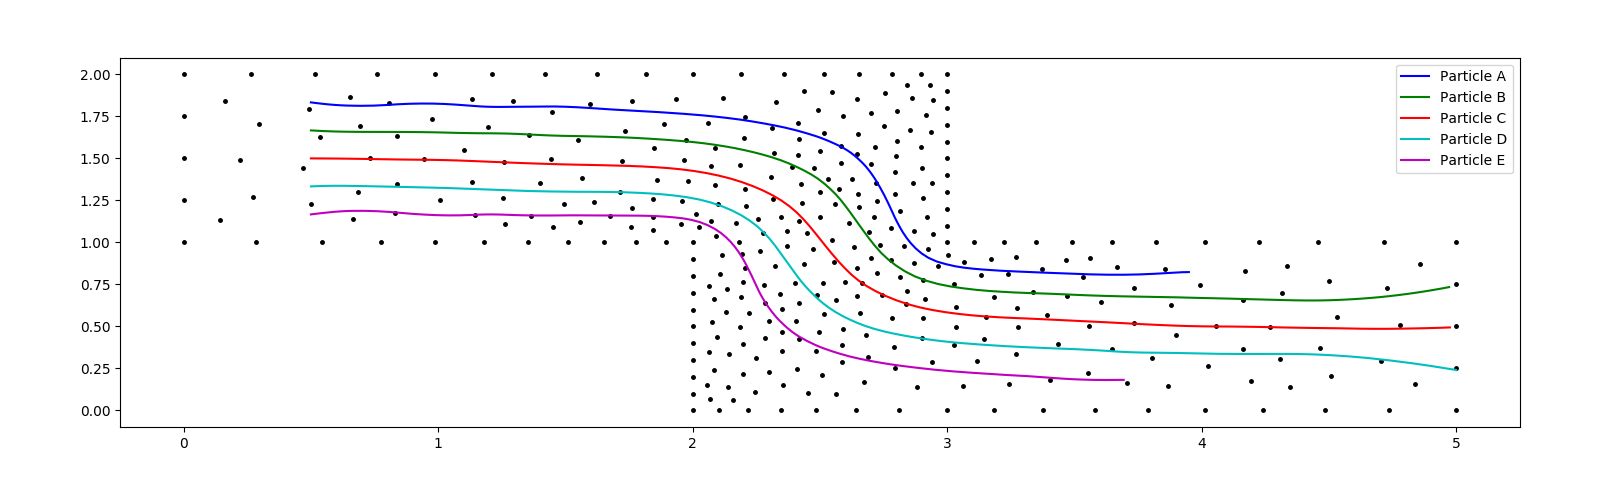
\includegraphics[width=\linewidth]{figures/Step_particle_trajectory.png}
    } {\raggedleft \scriptsize Fonte: Autor.}
    \caption{Trajeto de partículas inseridas em um escoamento com degrau.}
    \label{step_trajectory}
\end{figure}

Neste caso, pode-se notar que as partículas seguem a curva realizada pelo escoamento fielmente.
Caso as propriedades das partículas fossem alteradas poderia-se encontrar uma situação em que sua inércia fosse grande demais para fazer a curva a tempo e algumas colidiriam na parede. 

%------------------- Nozzle ----------------------------------
\section{\textbf{Simulação Em Um Canal Com Restrição}}
\label{sec_nozzle}
No escoamento com restrição há um aumento de velocidade na região restringida.
Isto ocorre devido à necessidade de aumentar o fluxo de fluido na região, de maneira a respeitar a Lei da Continuidade \eqref{continuity_final}.

As condições do escoamento são de um comprimento $L=10m$ com altura de entrada de $D_{entrada}=2m$ e uma entrada de saída de $D_{saida}=1m$.
O fluido entra com velocidade constante pela região da esquerda com velocidade $\vec{v}_{ent}=(1, 0)m/s$.
Nas paredes há a condição de não escorregamento, portanto a velocidade nas paredes inferior e superior são nulas, $\vec{v}_{sup}=\vec{v}_{inf}=0$.
Novamente a corrente possui uma condição de contorno variando de $0$ a $1$ nas bordas de acordo com sua posição, equivalente a $\psi_{cc}=y$.

Novamente, são incluidas as curvas de nível da velocidade na exibição do campo de velocidades na \ref{nozzle_result}:
\begin{figure}[H]
    \centering
    \stackunder{
        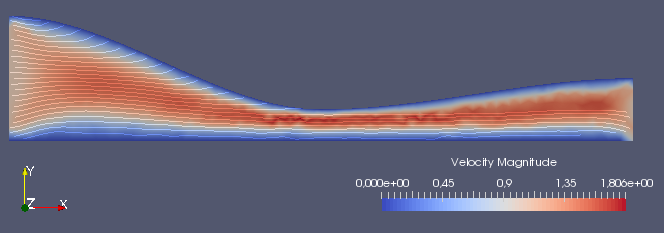
\includegraphics[width=\linewidth]{figures/Nozzle_result.png}
    } {\raggedleft \scriptsize Fonte: Autor.}
    \caption{Campo de velocidades de um escoamento com restrição.}
    \label{nozzle_result}
\end{figure}

Vizualizando-se os vetores do campo de velocidades, pode-se observar o aumento da velocidade na região restrita e uma componente vertical na velocidade elevado na região inicial do escoamento:
\begin{figure}[H]
    \centering
    \stackunder{
        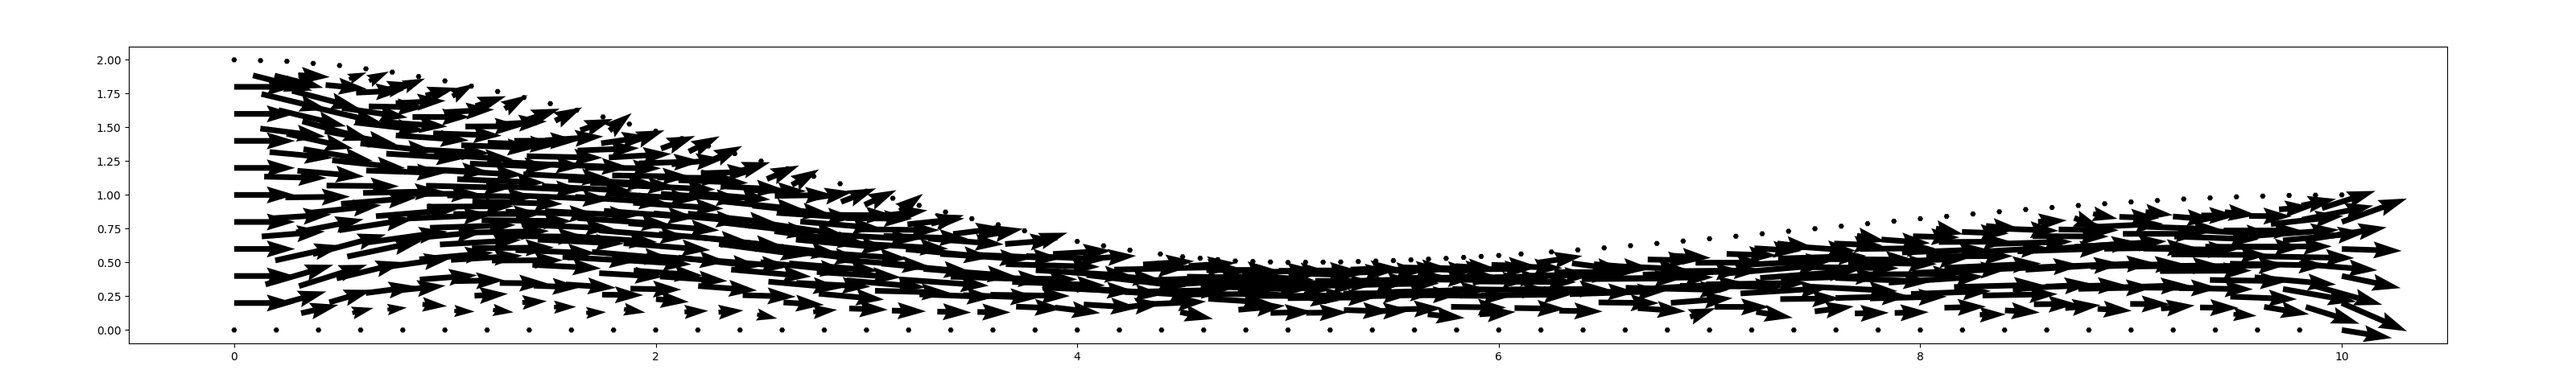
\includegraphics[width=\linewidth]{figures/Nozzle_velocity_field.png}
    } {\raggedleft \scriptsize Fonte: Autor.}
    \caption{Vetores de velocidades de um escoamento com restrição.}
    \label{nozzle_velocity}
\end{figure}

O trajeto das partículas realizado neste caso é demonstrado na \ref{nozzle_trajectory}:
\begin{figure}[H]
    \centering
    \stackunder{
        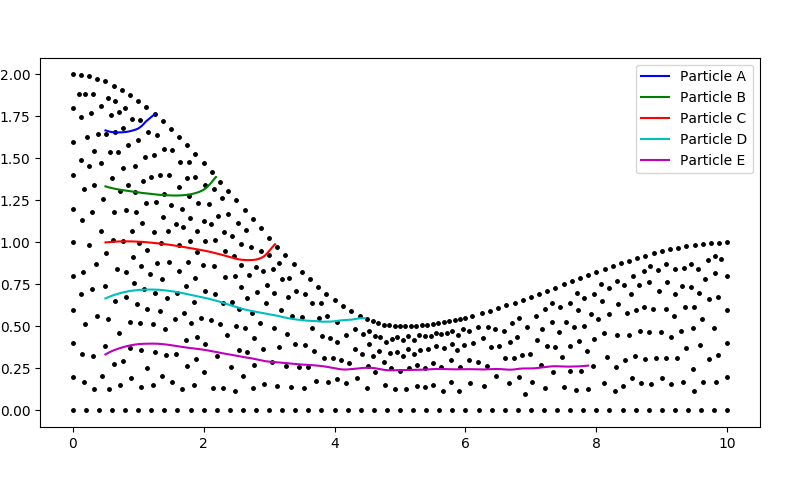
\includegraphics[width=\linewidth]{figures/Nozzle_particle_trajectory.png}
    } {\raggedleft \scriptsize Fonte: Autor.}
    \caption{Trajeto de partículas inseridas em um escoamento com restrição.}
    \label{nozzle_trajectory}
\end{figure}

Neste caso pode-se observar a colisão das partículas na extremidade superior logo após a entrada devido a uma corrente criada na região de entrada do escoamento.
Ao longo do canal, pode se observar que a partícula sofre uma aceleração ao atravessar a região restringida.

%------------------- Rotor -----------------------------------
\section{\textbf{Simulação Em Uma Pá de Rotor}}
\label{sec_rotor}
Finalmente, a simulação em uma pá de rotor visa representar o comportamento das partículas em uma situação real de trabalho de uma turbomáquina.
Foram feitas simulações para três tipos de partículas com diferentes materiais e diâmetros.
Foram utilizadas partículas de ouro com $\rho_{p,Au}=20000kg/m^3$ de densidade e $d_{p,Au}=1mm=1.10^{-3}m$ de diâmetro, de ferro, com $\rho_{p,Fe}=7300kg/m^3$ de densidade e $d_{p,Fe}=1mm=1.10^{-3}m$ de diâmetro, e de areia com $\rho_{p,Areia}=1600kg/m^3$ de densidade e $d_{p,Au}=0.5mm=5.10^{-4}m$ de diâmetro.
Com respeito ao tempo entre instantes, foram utilizados os intervalos de $dt=3.33e^{-5}s$ para a simulação com partículas de ouro, $dt=8.11e^{-6}s$, para a de ferro e $dt=4.44e^{-7}s$ para a de areia.
Já que quanto menor forem o tamanho e densidade das partículas torna-se necessário um intervalo para garantir a convergência.

A geometria pá foi extraida de um contorno de uma pá real de uma bomba exemplo, porém feitas em escala.
Foi tomado um arco na seção de entrada gerado com raio de $R_{ent}=0.5m$, e a saída com um arco de $R_{sai}=1.0m$.
A velocidade de entrada do fluido foi atribuída como $\vec{v}_{ent}=(0, 1)m/s$, no arco de entrada na região inferior.
Novamente, utiliza-se a condição de não escorregamento das paredes laterais, portanto na parede esquerda e direita tem-se$\vec{v}_{parede}=0$.
A função de corrente na parede esquerda é aplicada como $1$ e na direita como $0$.
Para a região de entrada, a corrente é tomada com valor crescente começando por $0$ no ponto coincidente com a parede direita até $1$ com o ponto presente na parede esquerda, similarmente é realizado o reciproco para a região de saída.

Neste trabalho, não serão levadas em conta as forças provenientes da rotação da máquina.
Portanto, é assumido que o domínio presente da pá é estacionário e é tomado como referência.

Novamente, são incluidas as curvas de nível da velocidade na exibição do campo de velocidades na \ref{rotor_result}:
\begin{figure}[H]
    \centering
    \stackunder{
        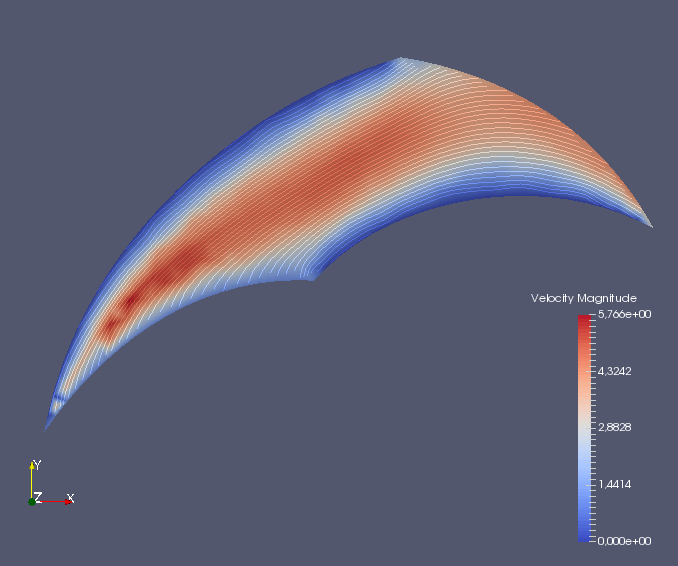
\includegraphics[width=\linewidth]{figures/Rotor_result.png}
    } {\raggedleft \scriptsize Fonte: Autor.}
    \caption{Campo de velocidades de um escoamento em uma pá de um rotor.}
    \label{rotor_result}
\end{figure}

E os vetores das velocidades nos nós:
\begin{figure}[H]
    \centering
    \stackunder{
        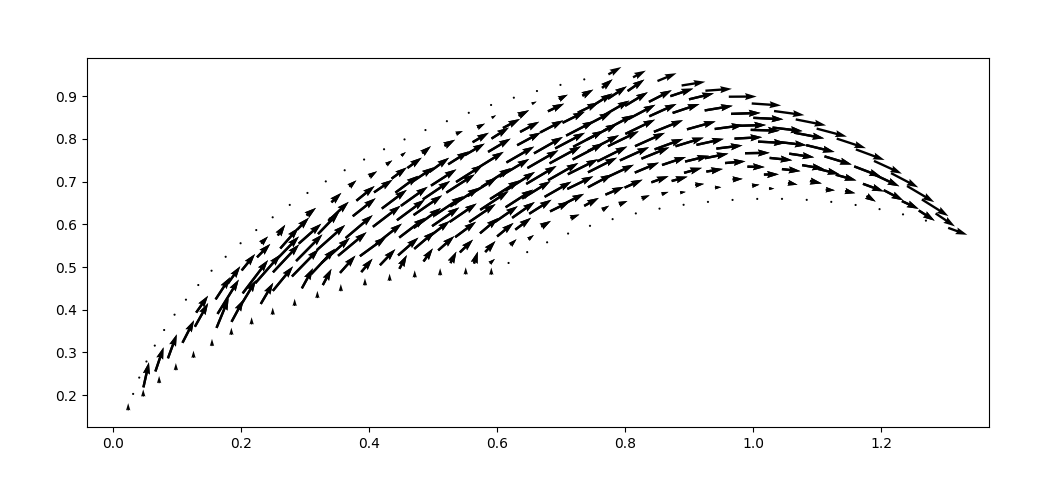
\includegraphics[width=\linewidth]{figures/Rotor_velocity_field.png}
    } {\raggedleft \scriptsize Fonte: Autor.}
    \caption{Vetores de velocidades de um escoamento em uma pá de um rotor.}
    \label{rotor_velocity}
\end{figure}

O resultado da simulação com as partículas de ouro na pá do rotor resultou no trajeto exibido na \ref{rotor_trajectory_gold}:
\begin{figure}[H]
    \centering
    \stackunder{
        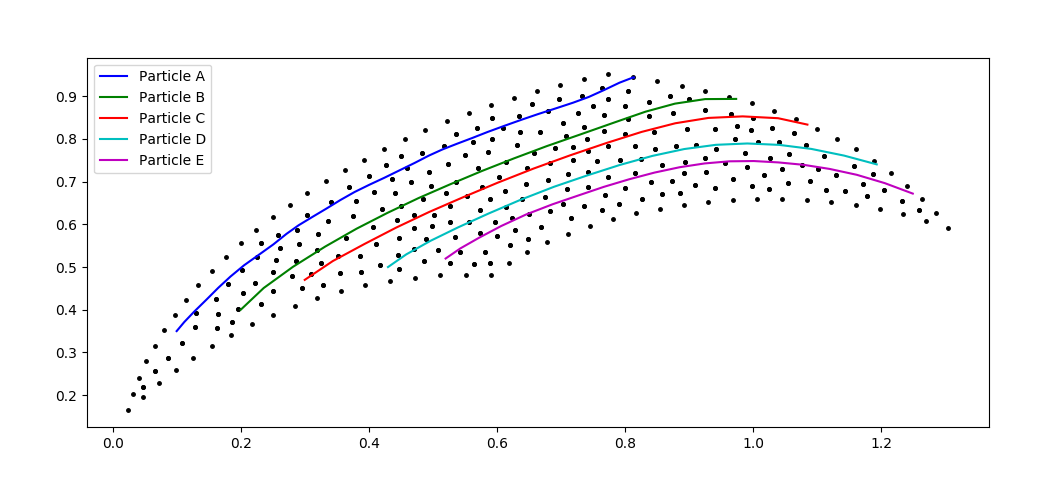
\includegraphics[width=\linewidth]{figures/Rotor_particle_trajectory_gold.png}
    } {\raggedleft \scriptsize Fonte: Autor.}
    \caption{Trajeto de partículas de ouro inseridas em um escoamento em uma pá de um rotor.}
    \label{rotor_trajectory_gold}
\end{figure}

Na simulação de partículas de ferro foi verificado o comportamento demonstrado na \ref{rotor_trajectory_iron}:
\begin{figure}[H]
    \centering
    \stackunder{
        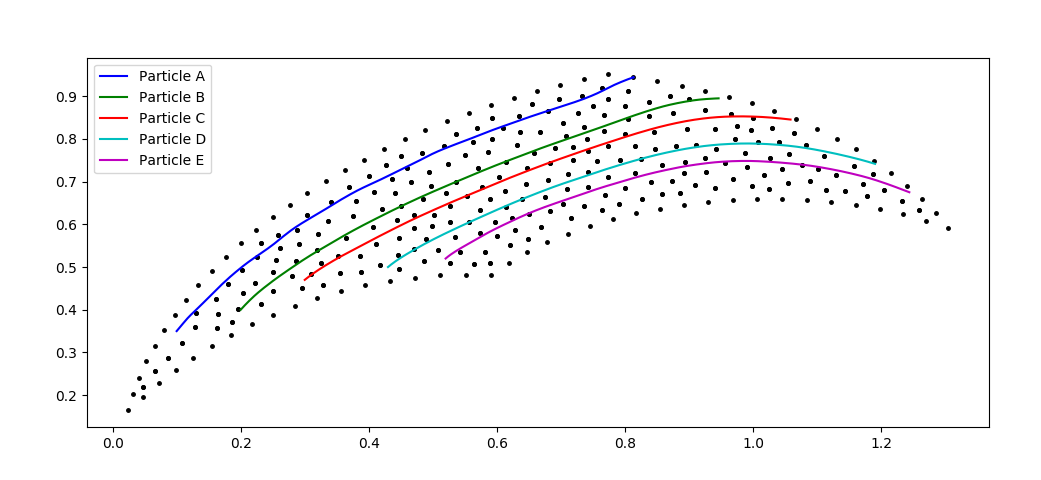
\includegraphics[width=\linewidth]{figures/Rotor_particle_trajectory_iron.png}
    } {\raggedleft \scriptsize Fonte: Autor.}
    \caption{Trajeto de partículas de ferro inseridas em um escoamento em uma pá de um rotor.}
    \label{rotor_trajectory_iron}
\end{figure}

E, finalmente, as partículas de areia realizaram a trajetória apresentada na \ref{rotor_trajectory_sand}:
\begin{figure}[H]
    \centering
    \stackunder{
        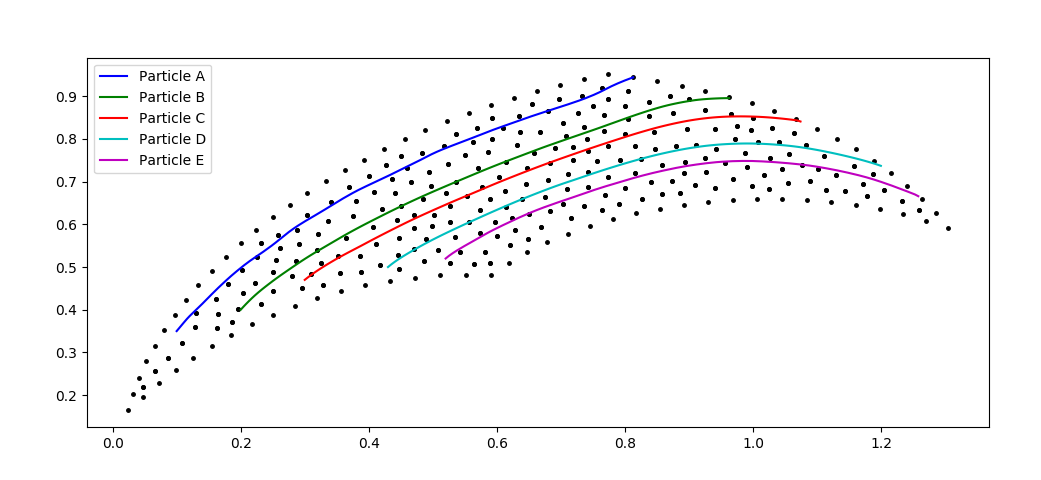
\includegraphics[width=\linewidth]{figures/Rotor_particle_trajectory_sand.png}
    } {\raggedleft \scriptsize Fonte: Autor.}
    \caption{Trajeto de partículas de areia inseridas em um escoamento em uma pá de um rotor.}
    \label{rotor_trajectory_sand}
\end{figure}

Pode-se observar que as partículas seguem ao longo geometria da pá, até mesmo a partícula mais distante acompanha as demais devido a uma região de velocidade elevada presente no canto esquerdo inferior.

As simulações com partículas mais leves levaram um tempo elevado para serem concluídas, devido a sua restrição no intervalo de cálculos.
Isto causou uma variação grande no tempo de cálculo das simulações, onde a simulação com partículas de ouro demorou em torno de 2h para ser completada, e as de ferro e areia demoraram em torno de 6h e 12h horas, respectivamente.